%!TEX root = ../thesis.tex
\chapter{Results}
\label{ch:results}
\begin{itemize}
    \item Unterteilung des Kapitels analog zur Fig. \ref{fig:Flowchart} in drei aufeinanderfolgende Abschnitte um Entscheidungen und Ergebnisse zu begründen
    \item mAP50-95 of all 5 Folds for every model
\end{itemize}
\section{Oriented Bounding Boxes and Axis Aligned Bounding Boxes}


\begin{figure}[h]
    \centering
    
    % Erste Zeile
    \begin{subfigure}[b]{0.45\textwidth}
        \centering
        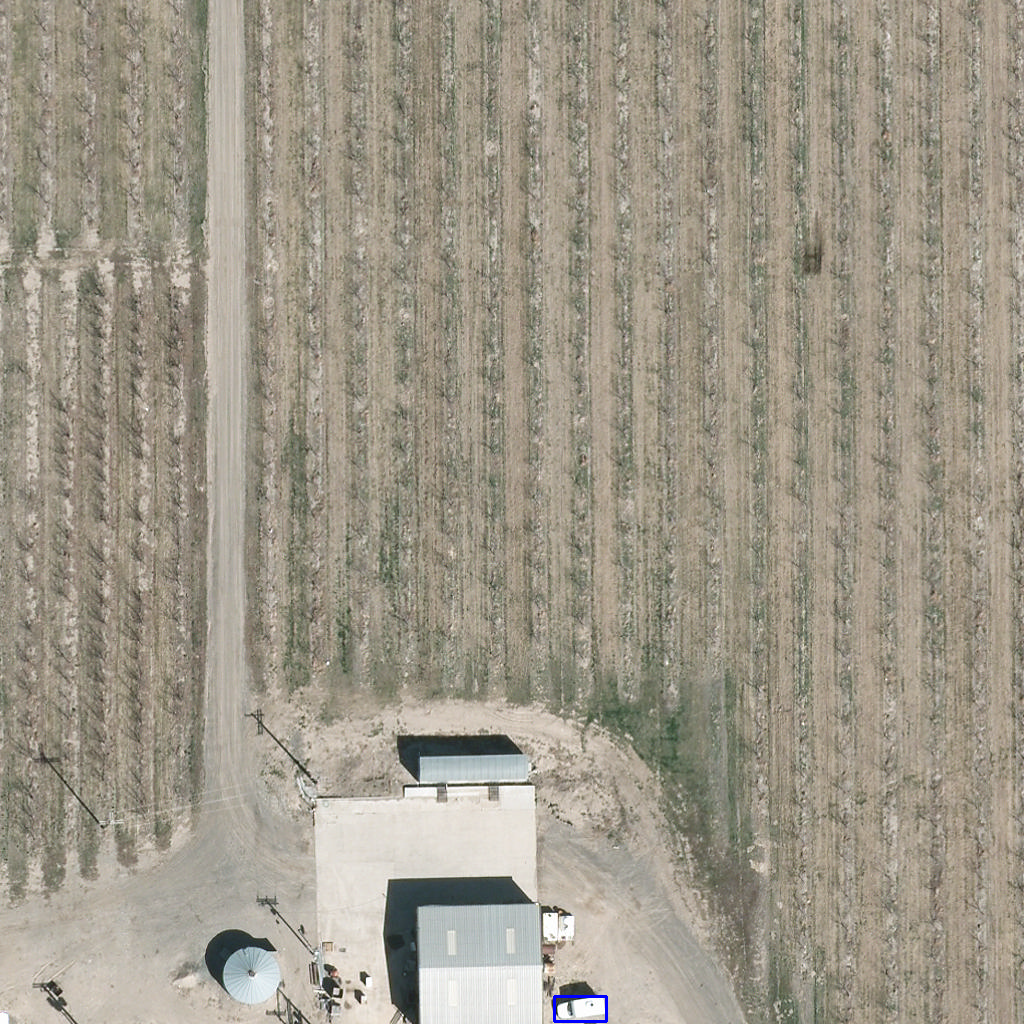
\includegraphics[trim={550pt 0pt 410pt 990pt},clip,width=\textwidth]{images/015Results/abb_vs_obb/abb_truck.png}
        \caption{Label: "Truck", abb format, area: $\approx 1378 \text{px}$}
        \label{fig:abb_truck}
    \end{subfigure}
    \hfill
    \begin{subfigure}[b]{0.45\textwidth}
        \centering
        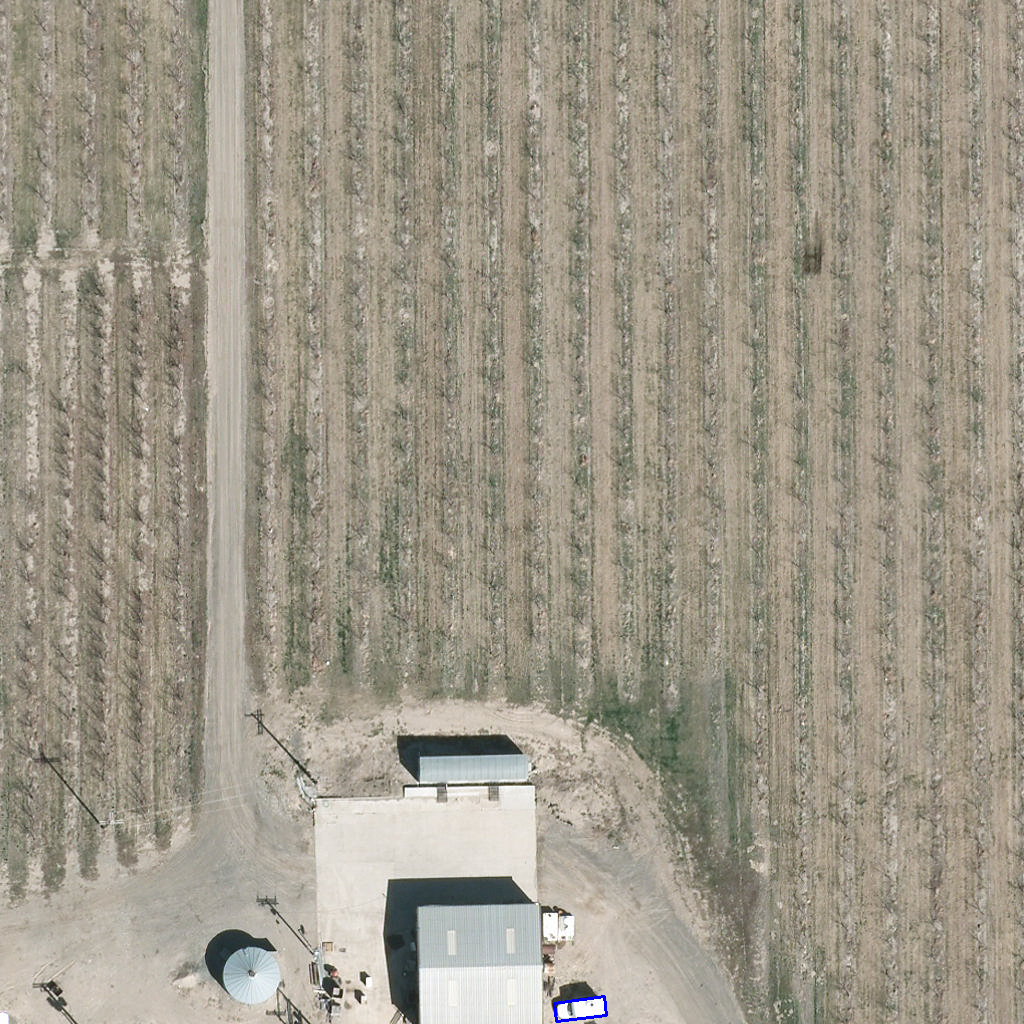
\includegraphics[trim={550pt 0pt 410pt 990pt},clip,width=\textwidth]{images/015Results/abb_vs_obb/obb_truck.png}
        \caption{Label: "Truck", obb format, area: $\approx 967 \text{px}$}
        \label{fig:obb_truck}
    \end{subfigure}
    
    \vspace{0.5cm} % Abstand zwischen den Zeilen
    
    % Zweite Zeile
    \begin{subfigure}[b]{0.45\textwidth}
        \centering
        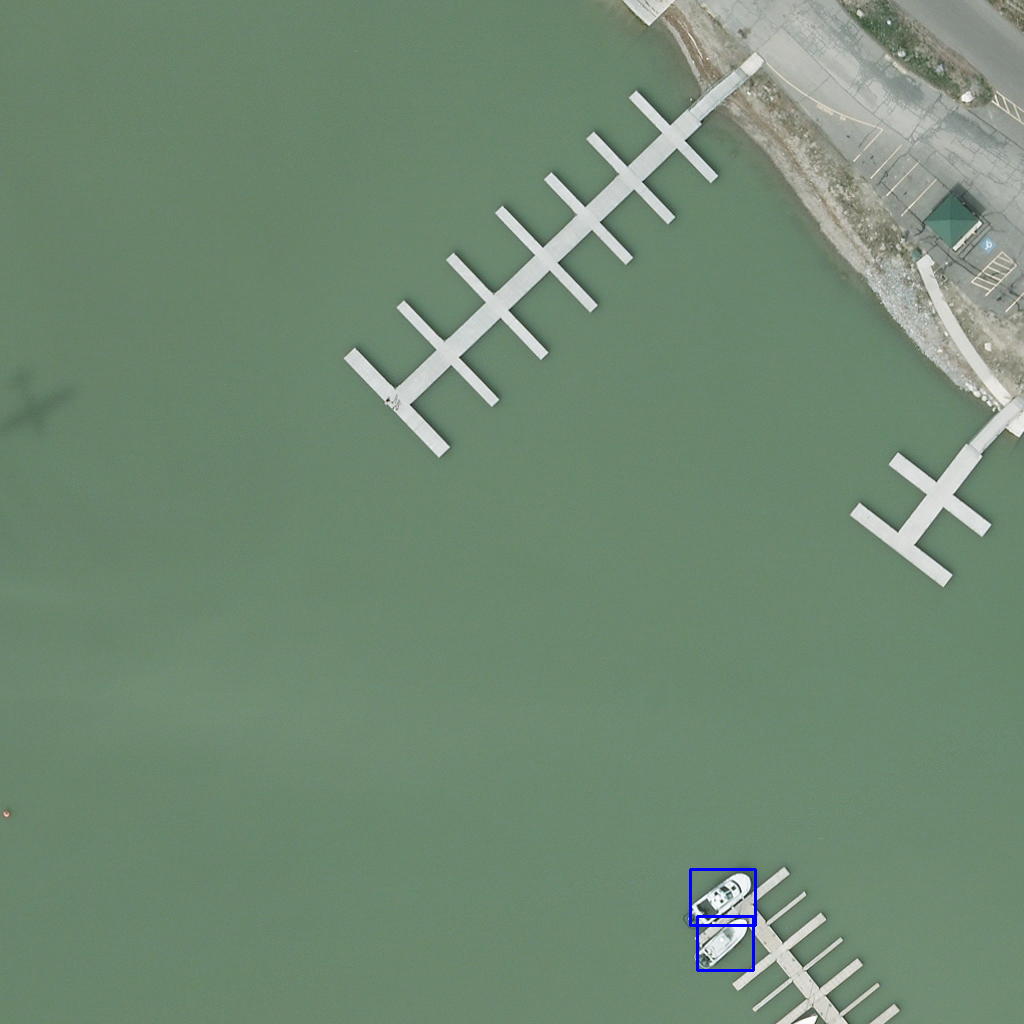
\includegraphics[trim={680pt 50pt 250pt 865pt},clip,width=\textwidth]{images/015Results/abb_vs_obb/abb_ship.png}
        \caption{Labels: "Ship", abb format}
        \label{fig:abb_ship}
    \end{subfigure}
    \hfill
    \begin{subfigure}[b]{0.45\textwidth}
        \centering
        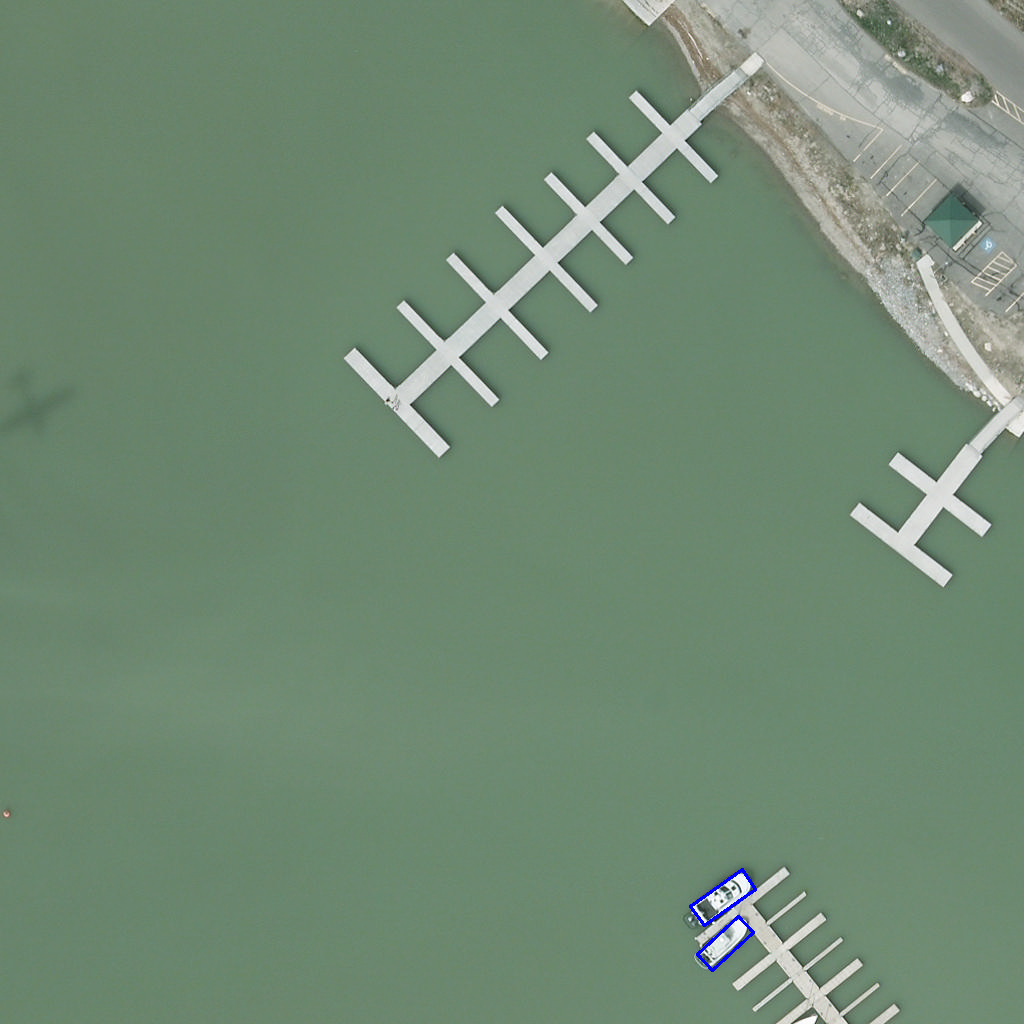
\includegraphics[trim={680pt 50pt 250pt 865pt},clip,width=\textwidth]{images/015Results/abb_vs_obb/obb_ship.png}
        \caption{Labels: "Ship", obb format}
        \label{fig:obb_ship}
    \end{subfigure}  
    \caption{Comparison of the bounding box formats of two different object classes}
    \label{fig:comparison_bb_format}
\end{figure}
\todo{nicht nur erläutern was man sieht sondern auch was man daraus folgert (analyse) im Bildunterschrift}


In Abbildung \ref{fig:comparison_bb_format} wird ein Vergleich zwischen \acrshort{obb} und \acrshort{abb} für verschiedene Objektklassen dargestellt. Besonders deutlich wird dieser Unterschied beim LKW-Beispiel: In Abbildung \ref{fig:abb_truck} nimmt die \acrshort{abb} mit ca. 1378 px eine deutlich größere Fläche ein als die \acrshort{obb} in Abbildung \ref{fig:obb_truck} mit ca. 967 px. Beim Vergleich stark rotierten Objekten, wie etwa bei den Schiffen in Abbildung \ref{fig:abb_ship} und \ref{fig:obb_ship}, zeigt sich, dass die \acrshort{obb} das Objekt selbst deutlich präziser umschließt und weniger umliegendes Areal einbezieht. Ein weiterer Vorteil der \acrshort{obb} ist das Fehlen von Überlappungen zwischen den Boxen.

Ein Vergleich aller Bounding Box-Flächen (vgl. Abbildung \ref{fig:bbox_area}) verdeutlicht, dass \acrshort{obb} im Mittel kompakter ist (Median \acrshort{abb}: ca. 1000 px, Median \acrshort{obb}: >700 px). Die \acrshort{abb}-Flächen entsprechen exakt den "abb in obb", da die Bounding Boxes identisch sind; der einzige Unterschied liegt im trainierten Modell. Die Bounding Boxen nehmen  als \acrshort{obb} (ca. 700 px pro Box) etwa 0,066\% der Gesamtfläche des Bildes ein, als \acrshort{abb} (ca. 1000 px pro Box) etwa 0,095\%. Damit liegen \acrshort{obb} knapp unterhalb der Untergrenze für sehr kleine Objekte nach \citeauthor{Chen2017} \cite{Chen2017} (s. Kap. \ref{ch:state_of_research}) und gelten als "very small objects", während \acrshort{abb} oberhalb der Untergrenze für kleine Objekte liegt und damit als "small object" gilt.


% \begin{itemize}
%     \item Zu sehen sind in Fig. \ref{fig:comparison_bb_format} ein Vergleich zwischen \acrshort{obb} und \acrshort{abb} bei verschiedenen Klassen
%     \item Fig. \ref{fig:abb_truck} hat mit ca. 1378 px als \Acrlong{abb} einen deutlich größere Fläche als die in \ref{fig:obb_truck} mit ca. 967 px
%     \item insbesondere beim vergleich der deutlich stärker rotierten \acrshort{BB} bei \ref{fig:obb_ship} und \ref{fig:abb_ship} ist zu sehen, dass die \acrshort{obb} sich deutlich stärker auf das Objekt selbst konzentriert und weniger umgebendes Areal umrandet. Ein weiterer wichtiger Punkt ist, dass keine Überlapppungen bei den \acrshortpl{obb} vorhanden ist.
%     \item  wenn man nun alle Bounding Box Areas vergleicht (s. Fig. \ref{fig:bbox_area}) ist zu sehen, dass obb deutlich kompatker (Median abb: ca. 1000 px, Median obb: >750 px) ist
%     \item \acrshort{abb} ist exakt gleich zu "abb in obb" da die \acrshort{BB} identisch sind ("abb in obb" hat die \acrshort{abb} bounding boxen ohne rotation)"; nur das Trainierte Modell unterscheidet sich
%     \item BB entsprechen der Definition von klein nach \cite{Chen2017}; nehmen als obb (700 px pro Box) ca, 0.066\% der Gesamtfläche des Bildes ein; und als abb (1000 px pro Box) 0.095\%; obb liegt damit knapp unterhalb der Untergrenze (very small object) und abb oberhalb der untergrenze (small object)
% \end{itemize}

\begin{figure}[htbp]
    \centering
    \includesvg[width=0.8\textwidth]{images/015Results/abb_vs_obb/boxplot_areas.svg}
    \caption[Comparison of Bounding Box Area in pixels for \acrshort{abb}, \acrshort{obb}, abb in obb]{Comparison of Bounding Box Area in pixels for \acrshort{abb}, \acrshort{obb}, abb in obb. "aab in obb" means, that \acrlong{abb} converted to obb was used in the \acrshort{YOLO}v9u model with zero rotation. (Own representation)}
    \label{fig:bbox_area}
\end{figure}


\begin{figure}[htbp]
    \centering
    \includesvg[width=0.8\textwidth]{images/015Results/abb_vs_obb/abb_obb_best_val_on_val.svg}
    \caption[Comparison of \acrshort{mAP}50-95 values for \acrshort{abb} and \acrshort{obb} (Best validation model on validation dataset)]{Comparison of \acrshort{mAP}50-95 values for \acrshort{abb} and \acrshort{obb} (Best validation model on validation dataset). "aab in obb" means, that \acrlong{abb} converted to obb was used in the \acrshort{YOLO}v9u model with zero rotation. (Own representation)}
    \label{fig:obb_abb_map50-95:val_on_val}
\end{figure}
Die Analyse der \acrshort{mAP}50--95 des besten Validierungsmodells auf dem Validierungsdatensatz (Abbildung \ref{fig:obb_abb_map50-95:val_on_val}) zeigt, dass das \acrshort{obb}-Modell in allen Fällen eine bessere Leistung erzielt als das \acrshort{abb}-Modell. Interessanterweise erzielt \acrshort{abb} auf dem \acrshort{obb}-Modell eine höhere Performance als die angepassten \acrshort{obb}-Boxen innerhalb desselben Modells (yolov9u). Dasselbe Phänomen lässt sich auch auf dem Testdatensatz beobachten (Abbildung \ref{fig:obb_abb_map50-95:test_on_val}), sodass \acrshort{abb} in Verbindung mit dem \acrshort{obb}-Modell bessere Ergebnisse liefert. Auffällig ist, dass bei den \acrshort{abb}-basierten Modellen (sowohl \acrshort{abb} als auch "abb in obb") stets Fold 1 den besten Wert beim besten Validation Dataset auf dem Validation Dataset erreicht hat, während beim \acrshort{obb}-Modell Fold 0 dort die besten Ergebnisse lieferte (s. Tab. \ref{tab:best_folds_area} und Fig. \ref{fig:obb_abb_map50-95:val_on_val}). Die Ergebnisse der jeweiligen Folds sind durch den roten Punkt in Abbildung \ref{fig:obb_abb_map50-95:test_on_val} gekennzeichnet. 
 Die Konsistenz über alle fünf Folds der Kreuzvalidierung ist gut, was auf eine robuste Trainierbarkeit der Modelle hinweist.

\begin{table}[h]
\centering
\begin{tabular}{l c}
\hline
\textbf{Model} & \textbf{Best Fold} \\
\hline
abb &  1 \\
obb &  0 \\
abb in obb &  1 \\
\hline
\end{tabular}
\caption{Best fold per model at Bounding Box format}
\label{tab:best_folds_area}
\end{table}

Aufgrund der geringeren Überlappungswahrscheinlichkeit und der genaueren Objektumrandung wurde das \acrshort{obb}-Modell für die weiteren Modelle im Rahmen der Permutationstests ausgewählt.
% \begin{itemize}
%     \item Wenn man nun die \acrshort{mAP}50-95 des besten Validerungsmodells auf dem Validierungsdatensatz betrachtet (s. Fig. \ref{fig:obb_abb_map50-95:val_on_val}), sieht man das das obb Modell in jedem Fall eine bessere Performance hat als das abb Modell
%     \item Unterschied im obb Modell ist zwischen den Bounding Box Formaten vorhanden; \acrshort{abb} hat auf dem obb Modell eine höhere Leistung als die eigentlich "besseren" / angepassten \acrshort{obb} auf dem obb Modell (yolov9u)
%     \item gleiches Phänomen ist auf dem Testdatensatz zu sehen (s. Fig. \ref{fig:obb_abb_map50-95:test_on_val})
%     \item \acrshort{abb} performt besser mit dem obb modell
%     \item Konsistenz aller Modelle über die 5 Folds der Kreuzvalidierung ist gut, was eine robuste Trainierbarkeit bedeutet
%     \item obb Modell für die Permutation entschieden, da Gefahr von Überlappungen geringer und genauere Umrandung der Objekte
% \end{itemize}

\begin{figure}[htbp]
    \centering
    \includesvg[width=0.8\textwidth]{images/015Results/abb_vs_obb/aab_obb_best_val_on_test.svg}
    \caption[Comparison of \acrshort{mAP}50-95 values for \acrshort{abb} and \acrshort{obb} (Best validation model on test dataset)]{Comparison of \acrshort{mAP}50-95 values for \acrshort{abb} and \acrshort{obb} (Best validation model on test dataset). "aab in obb" means, that \acrlong{abb} converted to obb was used in the \acrshort{YOLO}v9u model with zero rotation. The red dot is the fold, that has the best \acrshort{mAP}50-95 at the validation dataset (see fig. \ref{fig:obb_abb_map50-95:val_on_val}).(Own representation)}
    \label{fig:obb_abb_map50-95:test_on_val}
\end{figure}



% \begin{itemize}
%     \item Training Results by the mAP50-95 of all 5 Folds for every model 
%     \item Left Side (Blue): Yolov9 (without obb) and with axis aligned Bounding Boxes
%     \item Middle (Orange): Yolov9u with oriented bounding boxes
%     \item Uses Ultralytics as Backend for obb support
%     \item Right (Green): Yolov9u with axis aligned Bounding Boxes in the oriented Bounding Box format
%     \item Result -> aab performs better
%     \item \todo{Vergleichsbild eifnügen oder verweis}
%     \item This is probably due to the fact that small changes in the orientation of the bounding boxes lead to a greater deviation of the mean average precision 
%     \item Oriented Bounding boxes are smaller than the axis aligned bounding boxes -> higher inaccuracy of mAP50-95 (see next slide)
%     \item Red box at the right picture has a small deviation from the correct (blue) label
%     \item 
%     \item Konsistenz aller Modelle über die 5 Folds der Kreuzvalidierung ist gut, was eine robuste Trainierbarkeit bedeutet
% \end{itemize}
% \begin{itemize}
%     \item \todo{Bild für Vergleich der BB Area einfügen (zw. obb, aab aab old)}
%     \item Oriented Bounding Boxes has an area from around 600 to 900 pixels 
%     \item Axis aligned Bounding boxes from around 750 to 1300 px
%     \item-> higher inaccuracy of mAP50-95

%     \item For the channel permutation I used the obb model

% \end{itemize}

\section{Comparision at Mean Average Precision 50-95}
\begin{itemize}
    \item \todo{Bild einfügen best val dataset on val data}
    \item \todo{Tabelle einfügen  Comparison of best performed Fold by mAP50-95 (s. Defence)}
    \item See the performance of the best validation model on the validation data (per fold and model)
    \item RGBIR has the best performance followed by irgb 
    \item 3. place are rgb and rirb
    \item Rgir and both ndvi models has the poorest map values
\end{itemize}

\begin{itemize}
    \item \todo{Bild einfügen; best val dataset on test data}
    \item Best Validation Models on the test data (Fold 5)
    \item Red Dots are the best validation model at the validation data on the test data
    \item (means the highest whisker from the previous slide)
    \item Difference between the quantils, rgir performs at best
    \item Then the rirb model and rgb model 
\end{itemize}

\begin{itemize}
    \item \todo{Tabelle einfügen}
    \item Difference Between best mAP Fold at the validation data
    \item From 0 to 4
    \item Smaller difference at the mAP Performance at the test data
    \item Fold 2 and 3
    \item Now looking at the confusion and difference matrices
\end{itemize}



\section{Comparision with Confusion Matrices}
\begin{itemize}
    \item \todo{beide confusionsmatricen einfügen}
    \item Normalisierte Konfusions Matrix mit 9 Klassen und der Einteilung Background (Hintergrund)
    \item Right: Confusion Matric of RGBIR Modell on Fold 2:
    \item Good Performance at Cars, Trucks, Ships, Tractors, Camping Cars, Pick Up and planes
    \item Many confusion at vehicle with background
    \item Nearly the same for RGIR at Fold 3
    \item Both modells detected nearly all Planes
    \item Difference Matrics at next slide
\end{itemize}

\begin{itemize}
    \item \todo{Differenzmatrix RGBIR vs RGIR einfügen}
    \item At all Difference Matrices is red for the better performance of the RGBIR Model and blue for the other modell
    \item RGBIR detected Trucks, Ships and Tractor more accurate than the RGIR Model
    \item RGBIR seems more robust for common ground vehicles
    \item Both modells detect all planes (in short every modell detect all planes)
    \item Both modells misclassifier background as any class (RGBIR is better at vehicle and Camping Car) 
\end{itemize}

\begin{itemize}
    \item \todo{Differenzmatrix RGBIR vs RGB einfügen}
    \item RGBIR is better for detecting Ships (12\%) and Vehicles (15\%), slightliy degrades performance of car detection
    \item Vehicle is much better than in RGB Model (15\%)
    \item IR input helps for common vehicle recognition (vehicle includes Excavators, construction equipment, etc.)
    \item RGB is better in identifying ship and vehicle as background
\end{itemize}


\begin{itemize}
    \item \todo{Differenzmatrix RGBIR vs IRGB einfügen}
    \item RGBIR recognize Ships 21 \% better than the irgb model
    \item Particulary stronger for camping car and van classification (6\%)
    \item IRGB has more  background-ship and background-vehicle confusion
\end{itemize}

\begin{itemize}
    \item \todo{Differenzmatrix RGBIR vs RIRB einfügen}
    \item RGBIR detects Ships and vans better than RIRB Model
    \item RIRB misclassified van and ship as background more often than RGBIR

\end{itemize}


\begin{itemize}
    \item \todo{Differenzmatrix RGBIR vs GBNDBVI und RGBNDVI einfügen}
    \item RGBIR have a better performance in Ship, Tractor and Vehicle
    \item Both ndvi modells show  a tendency for confusing background with other classes
\end{itemize}

\section{Ablation Studies}
\begin{itemize}
    \item \todo{Tabelle mit Best Folds Ablation Studies einfügen}
\end{itemize}
% \begin{figure}[h] 
%     \centering
%     % Erste Subfigur
%     \begin{subfigure}[b]{0.85\textwidth} % [b] für bottom alignment, 0.48\textwidth damit noch Platz ist
%         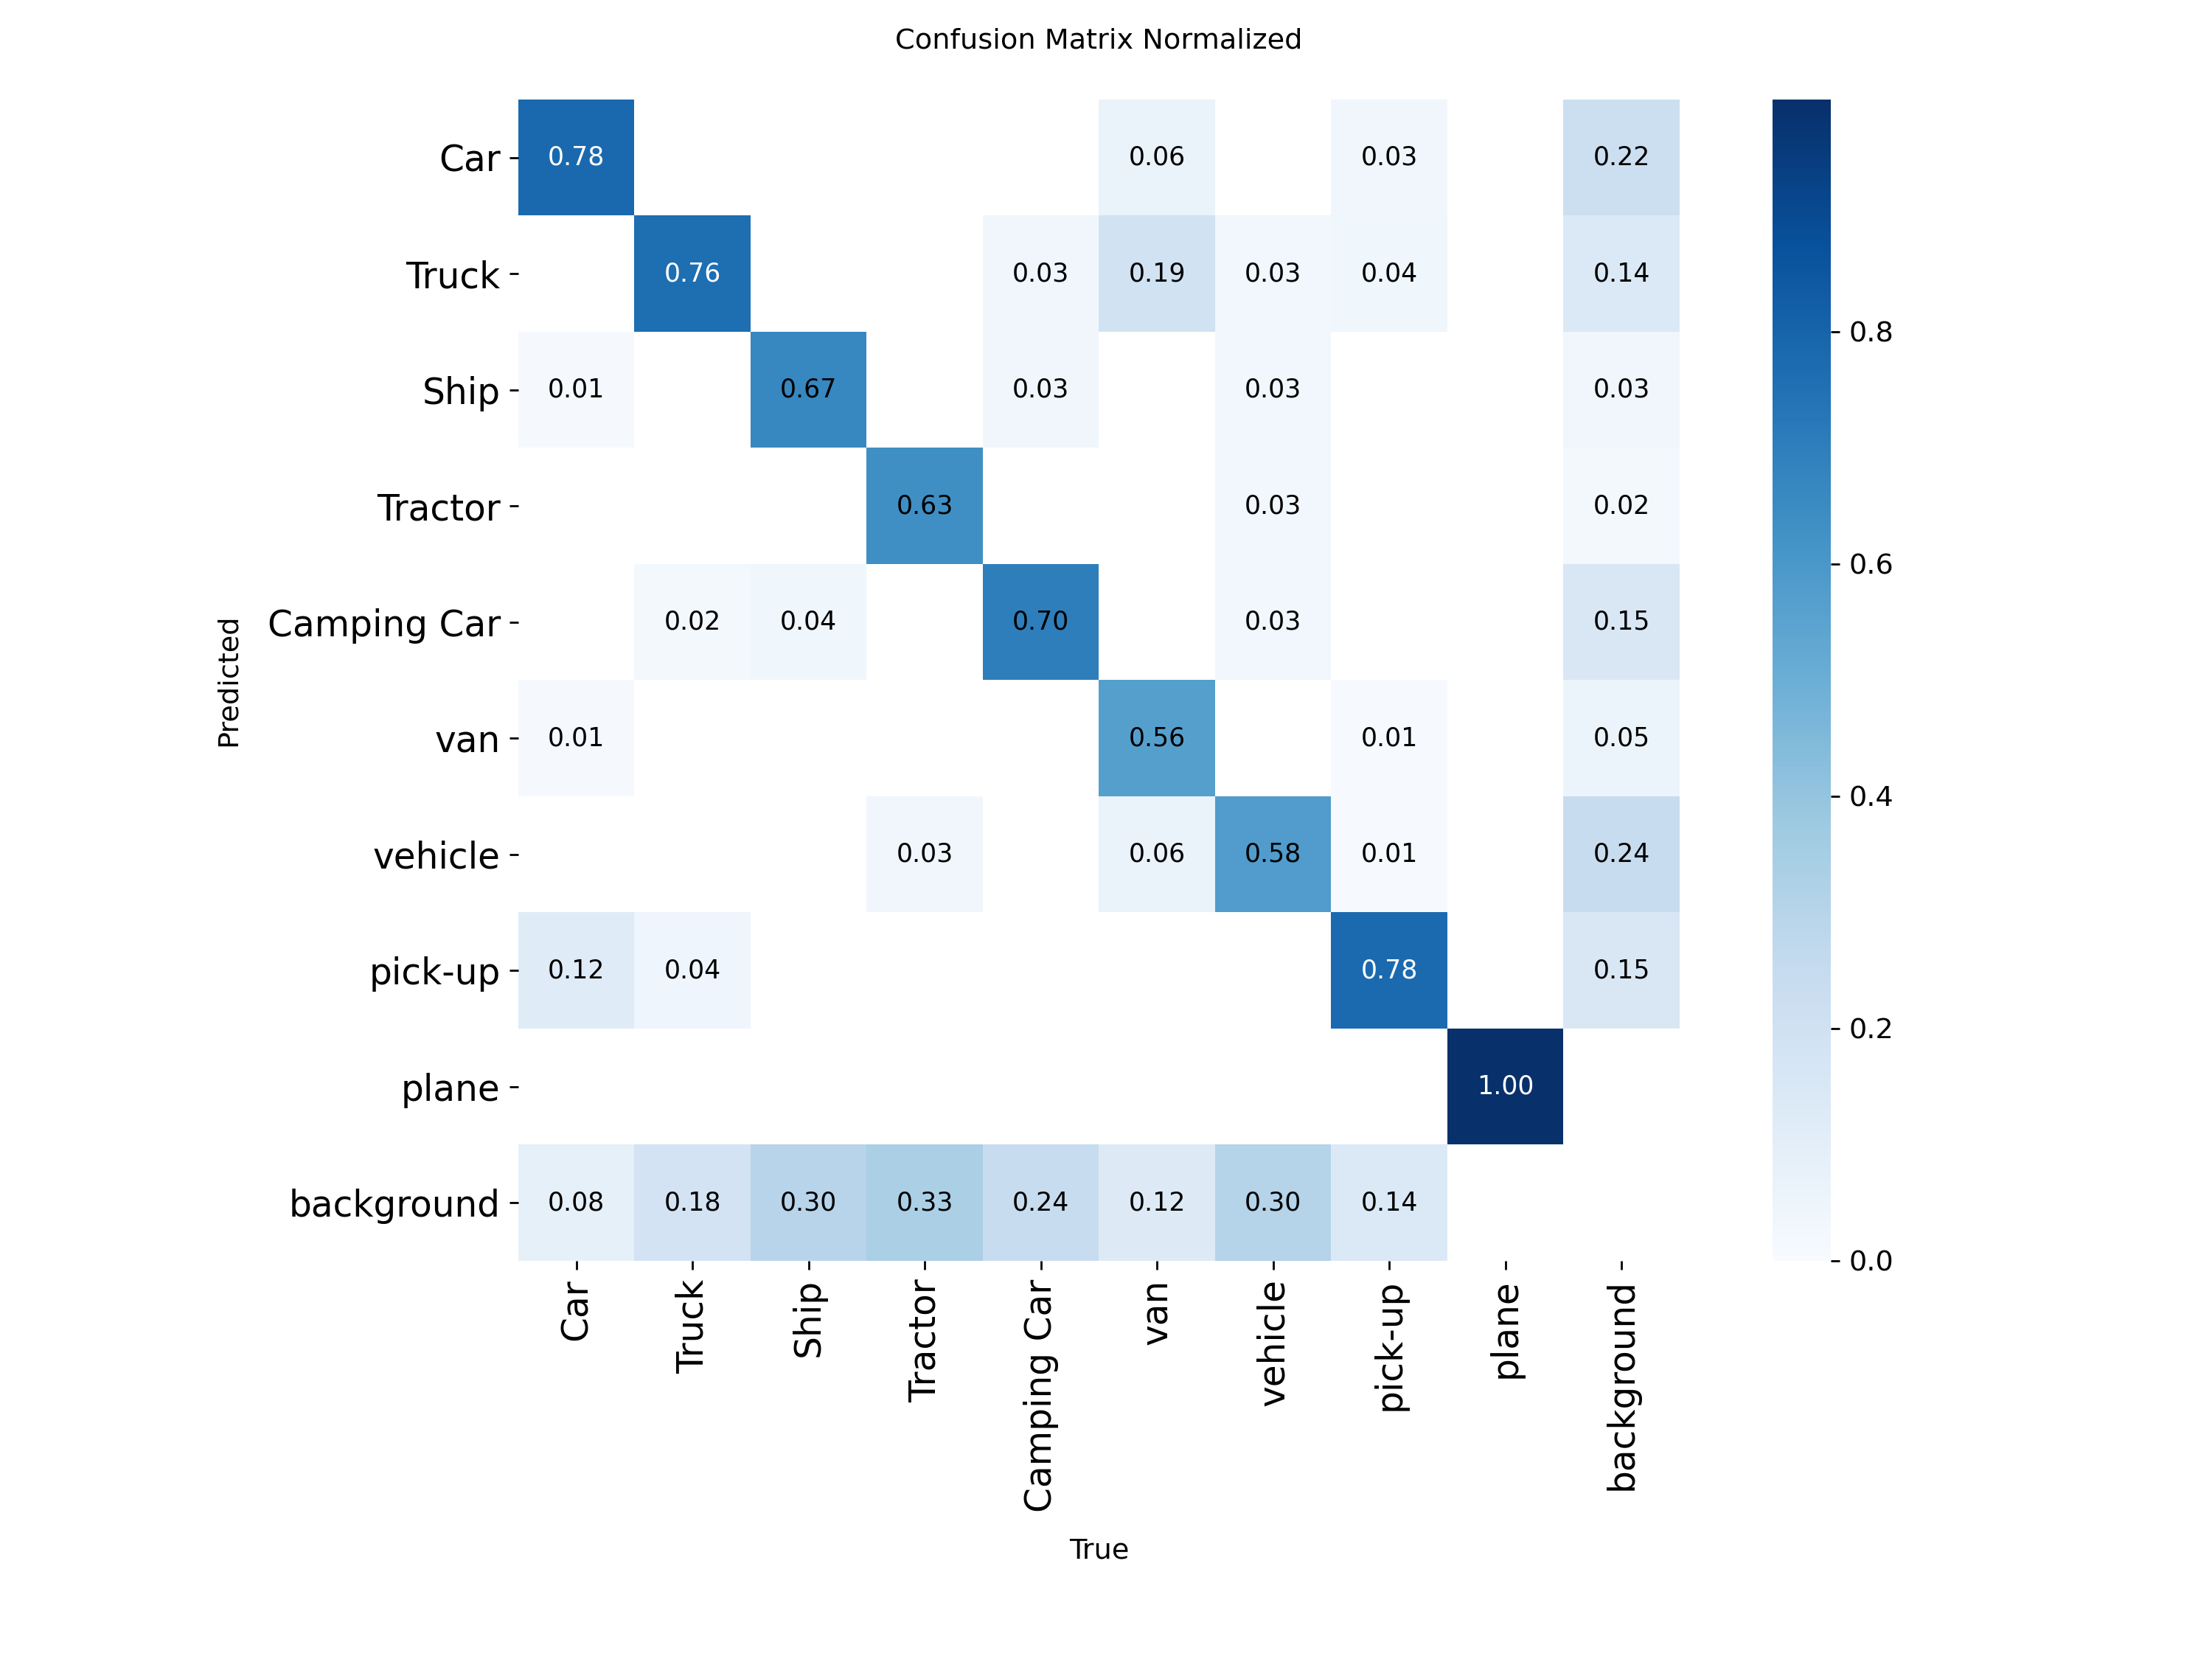
\includegraphics[width=\textwidth]{images/confusion_matrices/rgbir_F4_confusion_matrix_normalized.png} % Bildpfad zum ersten Bild
%         \caption{r-g-b-ir} % Unterschrift für das erste Bild
%         \label{fig:cm_rgbir} % Label für Referenzierung von Bild 1
%     \end{subfigure}
%     \hfill % Fügt horizontalen Platz zwischen den Subfiguren ein
%     % Zweite Subfigur
%     \begin{subfigure}[b]{0.85\textwidth} % 0.48\textwidth für das zweite Bild
%         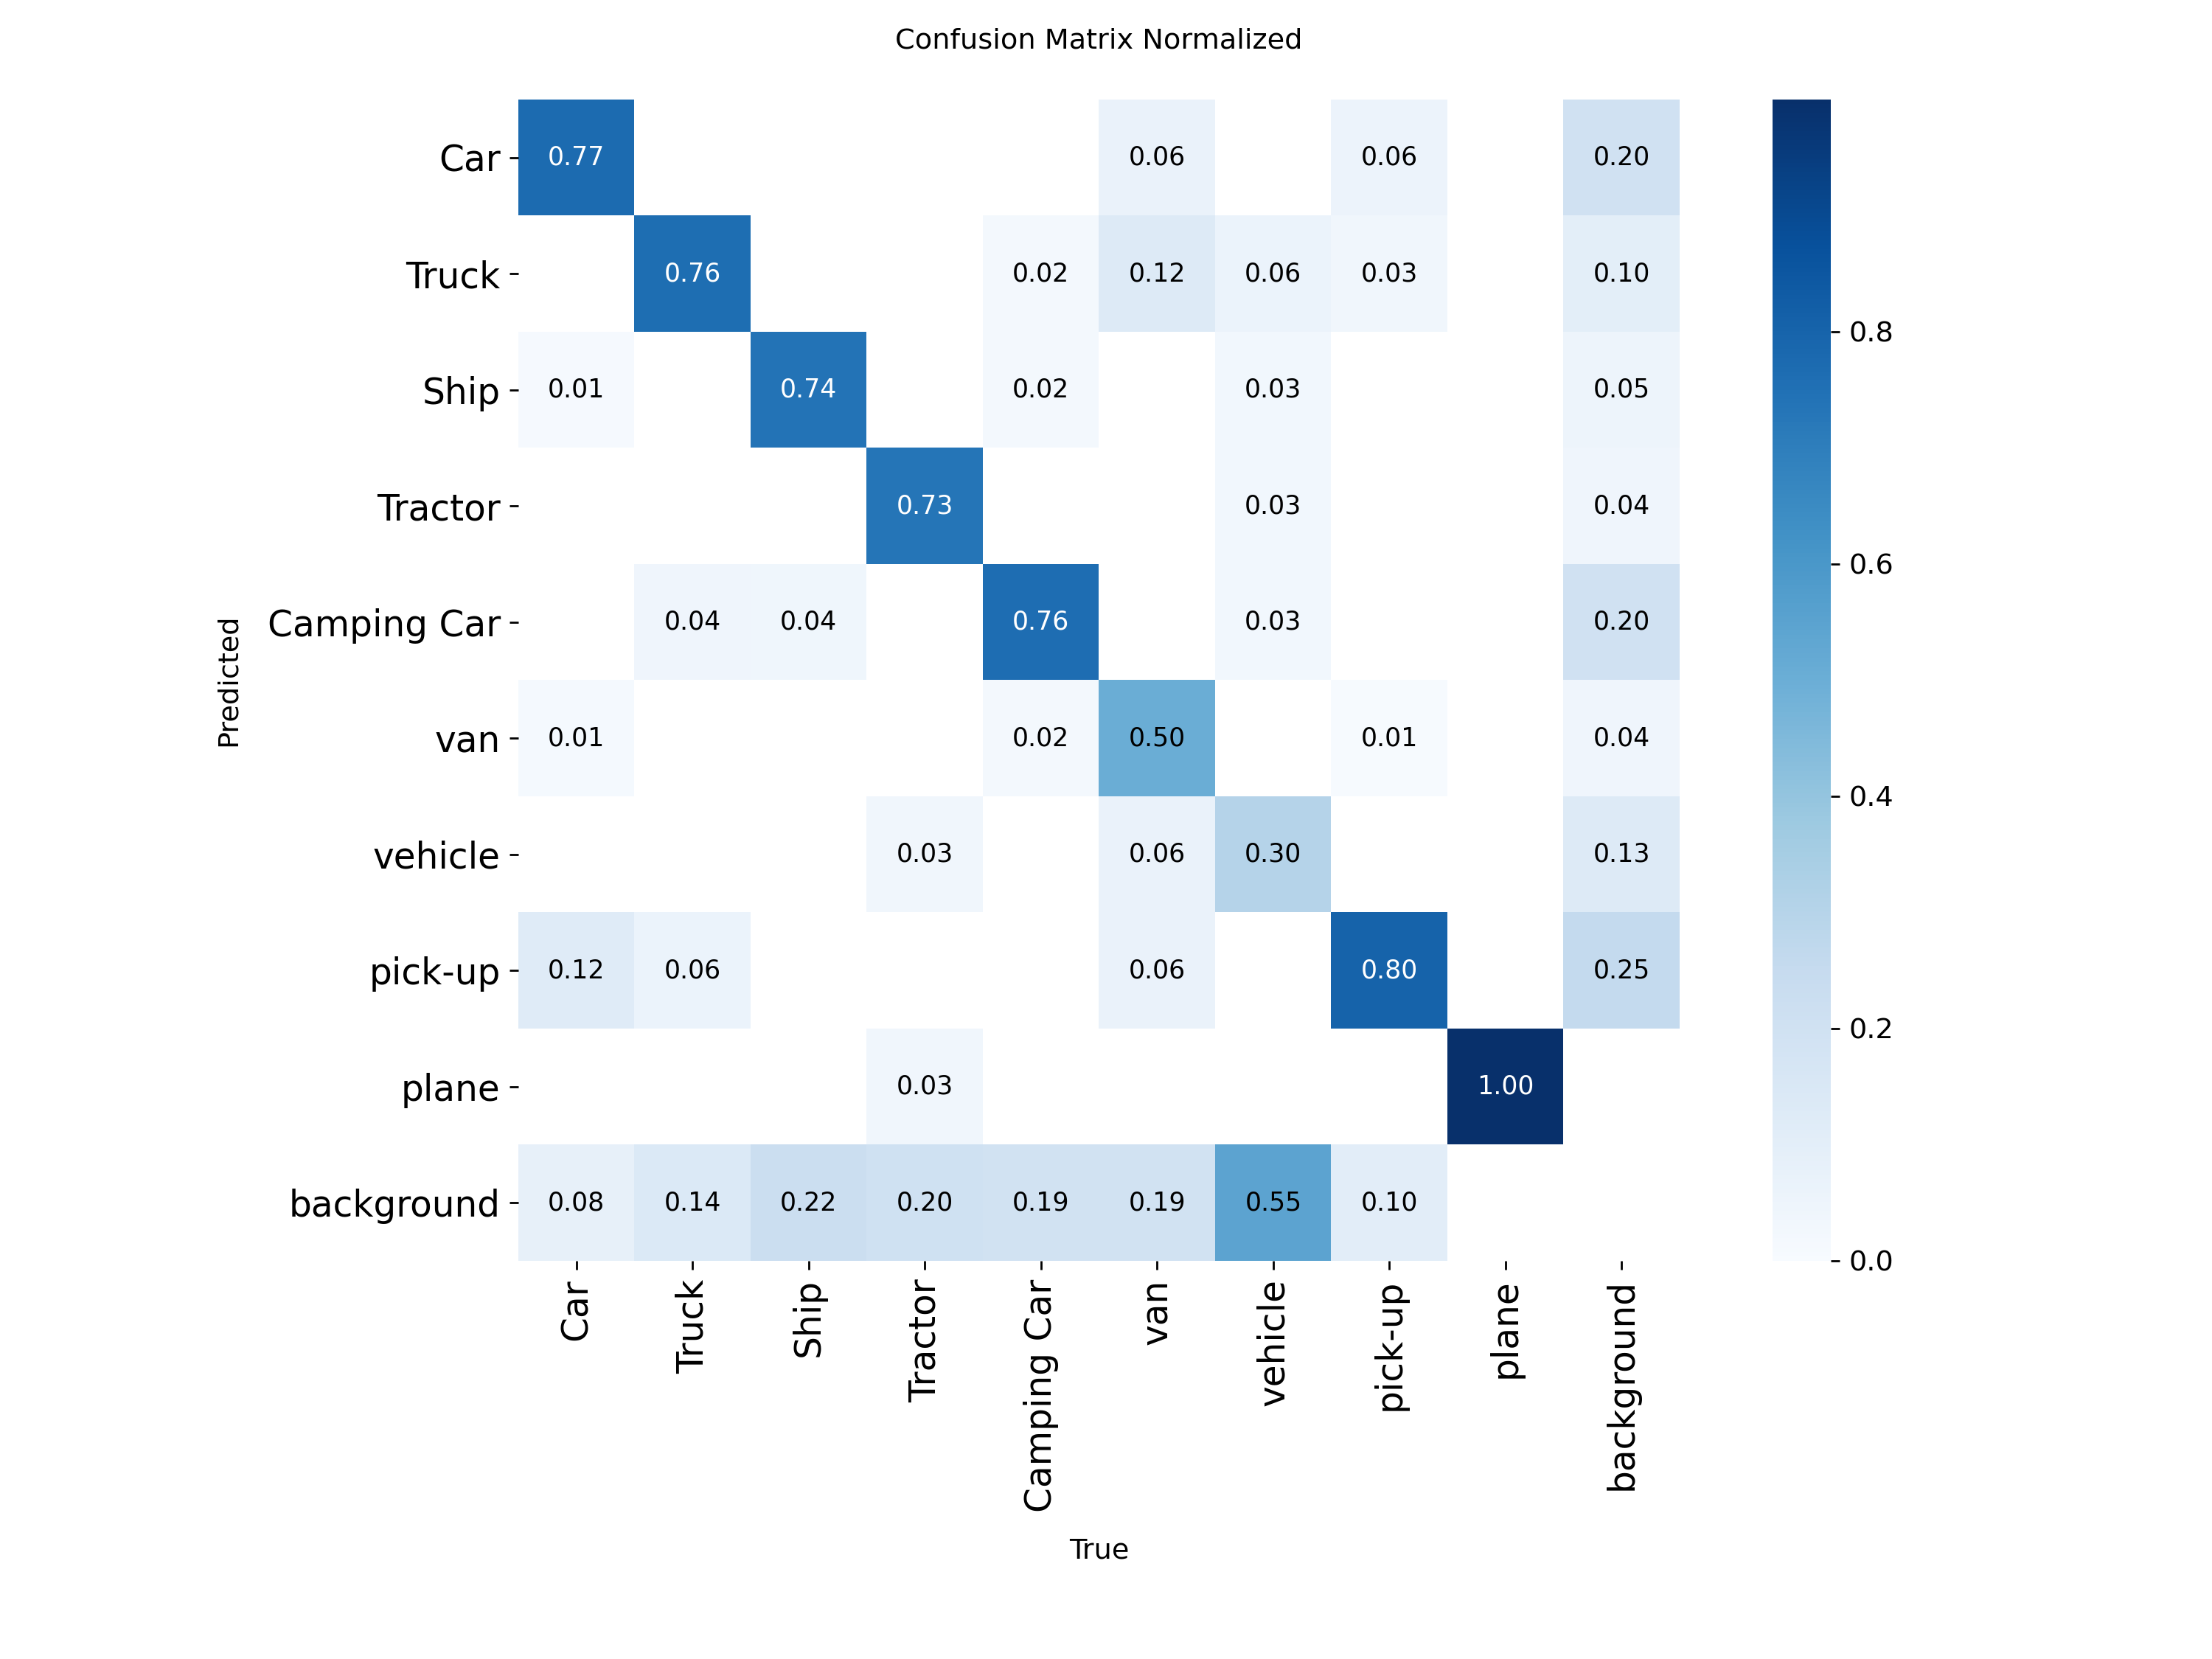
\includegraphics[width=\textwidth]{images/confusion_matrices/irgb_F4_confusion_matrix_normalized.png} % Bildpfad zum zweiten Bild
%         \caption{ir-g-b} % Unterschrift für das zweite Bild
%         \label{fig:cm_irgb} % Label für Referenzierung von Bild 2
%     \end{subfigure}
%     \caption{Comparison of Confusion Matrices between r-g-b-ir und ir-g-b for Fold 4} % Gemeinsame Unterschrift für beide Bilder
%     \label{fig:combined_maps} % Label für die gesamte Figure-Umgebung
% \end{figure}

% \begin{figure}[h] 
%     \centering
%     % Erste Subfigur
%     \begin{subfigure}[b]{0.85\textwidth} % [b] für bottom alignment, 0.48\textwidth damit noch Platz ist
%         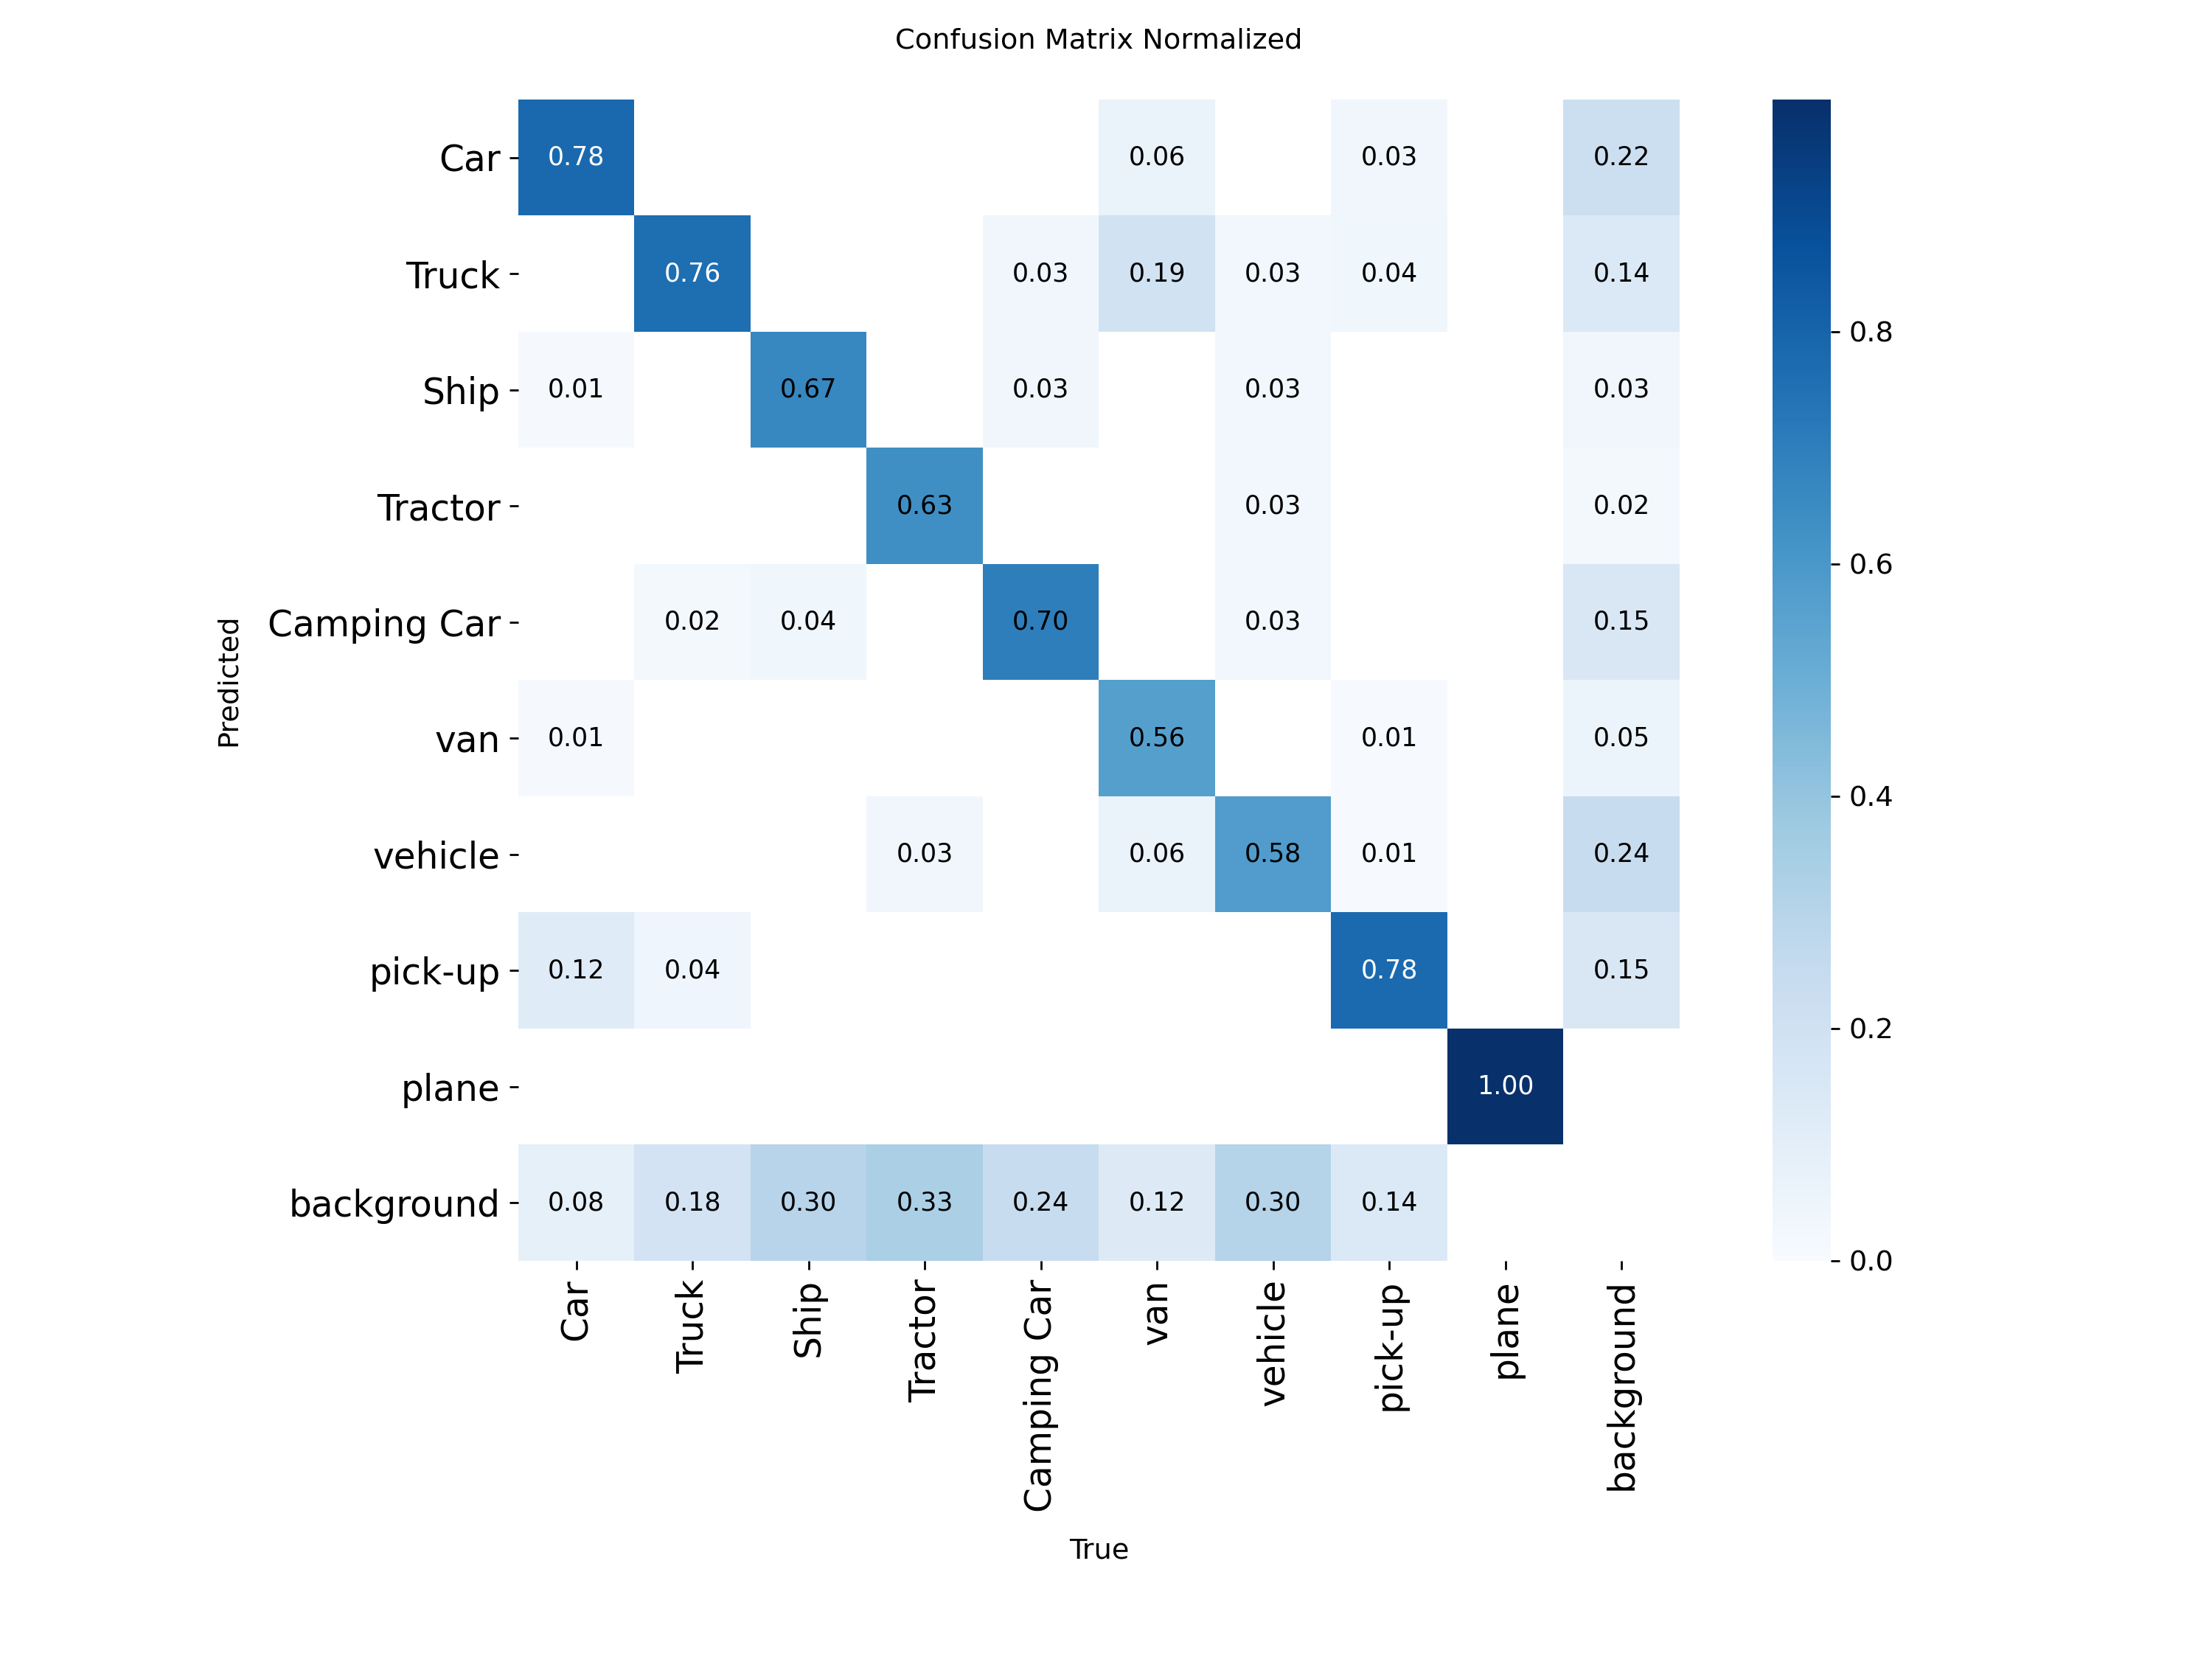
\includegraphics[width=\textwidth]{images/confusion_matrices/rgbir_F4_confusion_matrix_normalized.png} % Bildpfad zum ersten Bild
%         \caption{r-g-b-ir} % Unterschrift für das erste Bild
%         \label{fig:cm_trgbir} % Label für Referenzierung von Bild 1
%     \end{subfigure}
%     \hfill % Fügt horizontalen Platz zwischen den Subfiguren ein
%     % Zweite Subfigur
%     \begin{subfigure}[b]{0.85\textwidth} % 0.48\textwidth für das zweite Bild
%         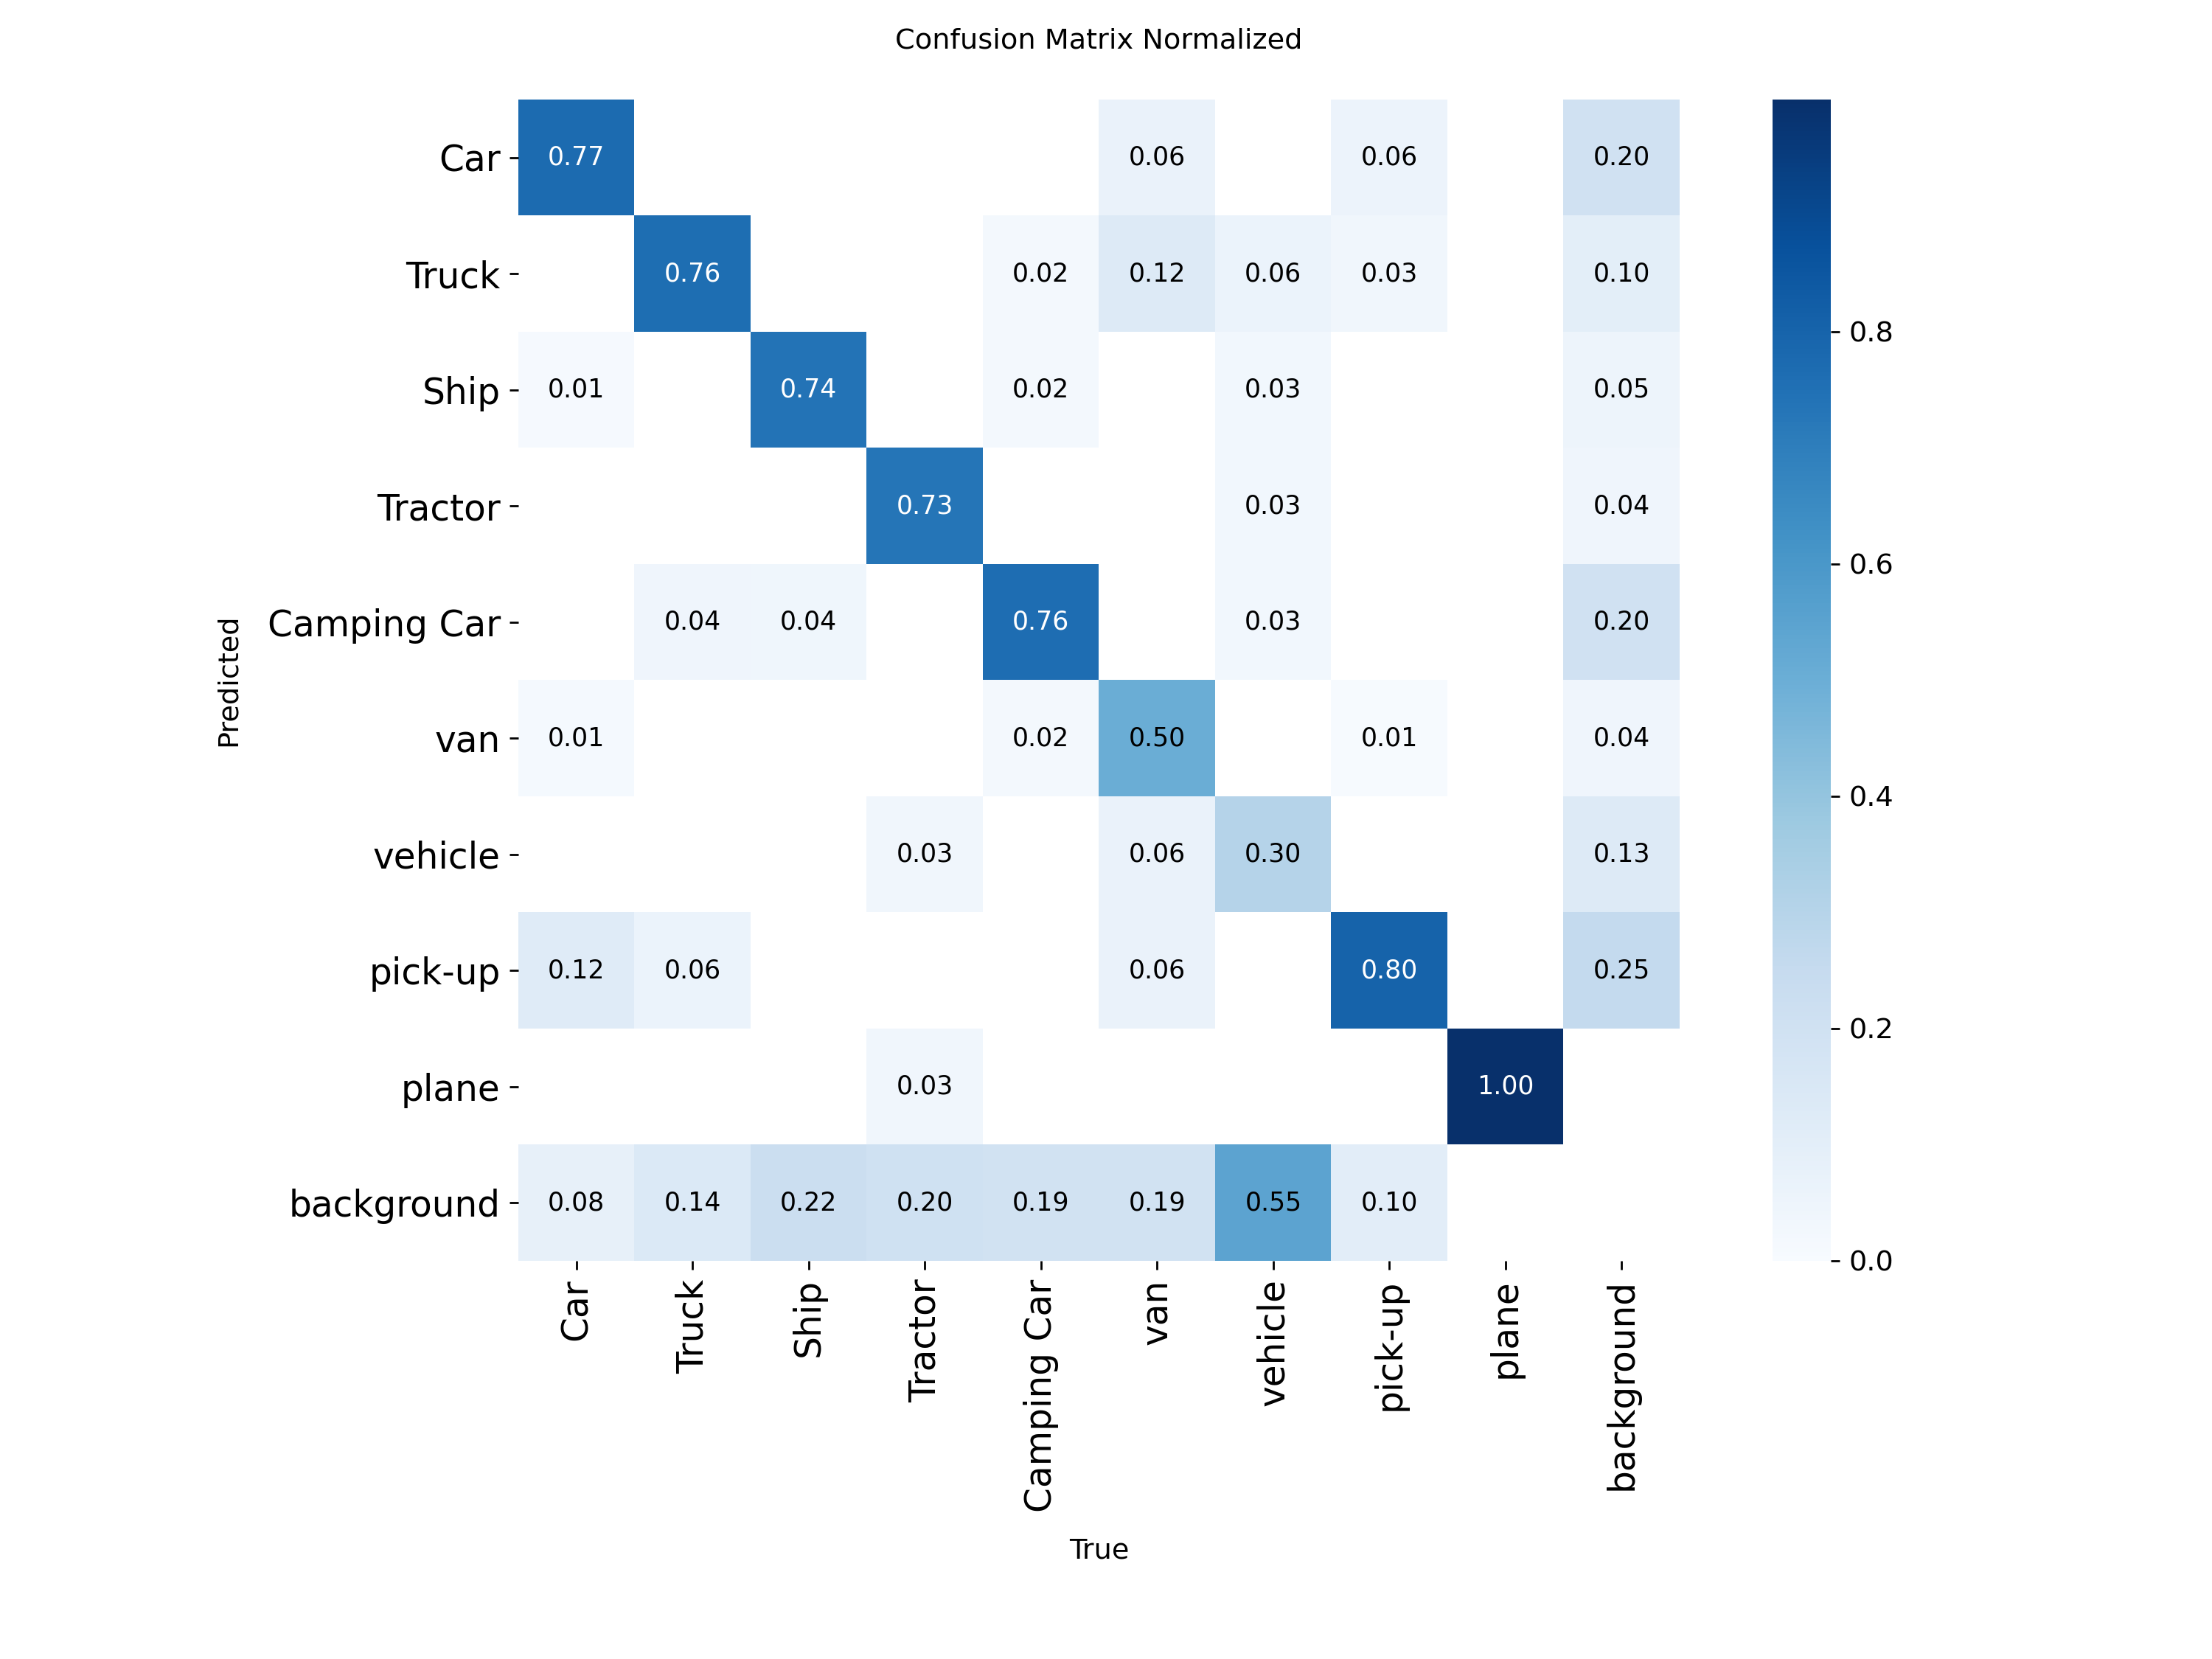
\includegraphics[width=\textwidth]{images/confusion_matrices/irgb_F4_confusion_matrix_normalized.png} % Bildpfad zum zweiten Bild
%         \caption{ir-g-b} % Unterschrift für das zweite Bild
%         \label{fig:cm_irgb} % Label für Referenzierung von Bild 2
%     \end{subfigure}
%     \caption{Comparison of Confusion Matrices between r-g-b-ir und ir-g-b for Fold 4} % Gemeinsame Unterschrift für beide Bilder
%     \label{fig:combined_maps} % Label für die gesamte Figure-Umgebung
% \end{figure}